\section{Parciální derivace}

\subsection{Výpočet pomocí vzorců}

Vypočtěte následující parciální derivace

\newcommand\pd[2][x]{\frac{\partial }{\partial #1}\left(\vphantom {\frac 22}#2\right)}
\begin{multicols}2
\begin{enumerate}[a)]
\item $\pd{x^2y+2xy^3+x+1}$
\item $\pd[y]{x^2y+2xy^3+x+1}$
\item $\pd{3x(3-x-2y)}$
\item $\pd[y]{3x(3-x-2y)}$
\item $\pd[x]{\sqrt{1-x^2-y^2}}$
\item $\pd[y]{\sqrt{1-x^2-y^2}}$
\item $\pd[x]{\frac x{x^2+y^2}}$
\item $\pd[y]{\frac x{x^2+y^2}}$
\end{enumerate}
\end{multicols}

\reseni
\begin{enumerate}[a)]
\item $\pd{x^2y+2xy^3+x+1}=2x\cdot y+2y^3+1+0=2xy+2y^3+1$
\item $\pd[y]{x^2y+2xy^3+x+1}=x^2+2x\cdot 3y+0+0=x^2+6xy$
\item $\pd{3x(3-x-2y)}=\pd{9x-3x^2-6xy}=9-3\cdot 2x-6\cdot 1\cdot y=9-6x-6y$
\item $\pd[y]{3x(3-x-2y)}=\pd[y]{9x-3x^2-6xy}=0-0-6x=-6x$
\item $\cdots=\pd[x]{(1-x^2-y^2)^{\frac 12}}=\frac 12 (1-x^2-y^2)^{-\frac 12} (0-2x-0)=
  \frac {x}{\sqrt{1-x^2-y^2}}$
\item $\cdots=\pd[y]{\sqrt{1-x^2-y^2}}= \frac {y}{\sqrt{1-x^2-y^2}}$ (z předchozího výpočtu a symetrie)
  
\item $\pd[x]{\frac x{x^2+y^2}}=\frac{1(x^2+y^2)-x(2x+0)}{(x^2+y^2)^2}=\cdots$ (derivace podílu)
\item $\pd[y]{\frac x{x^2+y^2}}=\pd[y]{x(x^2+y^2)^{-1}}=x(-1)(x^2+y^2)^{-2}(0+2y)=\cdots$ (derivace konstantního násobku mocninné funkce s vnitřní složkou)

\end{enumerate}


\konec


\obrazek{blizzard.jpg}

\subsection{Parciální derivace, pocitová teplota analyticky}
\shorthandoff{-}

Kanadský empirický vzorec pro pocitovou teplotu v zimě (wind chill factor) je
$$
%\begin{dmath*}
\begin{aligned}
W(T,v) = &13.12+0.6215 T-11.37 v^{0.16}\\&+0.3965 T v^{0.16},
\end{aligned}
%\end{dmath*}
$$
kde $T$ je teplota
(ve stupních Celsia) a $v$ je rychlost větru (v km/hod). Teplota je $-11.0\,{}^\circ\!\text{C}$  a rychlost větru $26
\,\text{km/hod}$. Určete parciální derivace pocitové teploty podle skutečné teploty a podle rychlosti větru (včetně jednotky) a výsledky interpretujte slovně.

\reseni

Dosazením do vzorce dostáváme $W(-11,26)=-20.212\,{}^\circ\!\text{C}$. Derivováním dostáváme
$$\begin{aligned}\frac{\partial W}{\partial T}(T,v)&=0.6215+0.3965 v^{0.16},\\
\frac{\partial W}{\partial v}(T,v)&=-11.37\times 0.16 v^{-0.84}+0.3965 \times 0.16 Tv^{-0.84}
\end{aligned}
$$
a po dosazení
$$\begin{aligned}\frac{\partial W}{\partial T}(-11,26)&=1.289,\\
\frac{\partial W}{\partial v}(-11,26)&=-0.163 \,{}^\circ\!\text{C}\, /(\mathrm{km}\, \text{hod}^{-1})=-0.163 \,{}^\circ\!\text{C}\, \text{hod} \,\mathrm{km}^{-1}.
\end{aligned}
$$
Za dané teploty a rychlosti větru je pocitová teplota $-20.2$ stupňů
Celsia. Nárůst teploty o jeden stupeň způsobí nárůst pocitové teploty
přibližně o $1.3$ stupně. Tedy změna teploty se projeví na pocitové
teplotě $1.3$-násobkem, tj. každkouzměnu vnímáme o třicet procent
intenzivněji.

Podobně, zesílení větru o jeden kilometr za hodinu způsobí snížení
pocitové teploty přibližně o $0.16$ stupně.

\konec

\subsection{Pocitová teplota numericky}

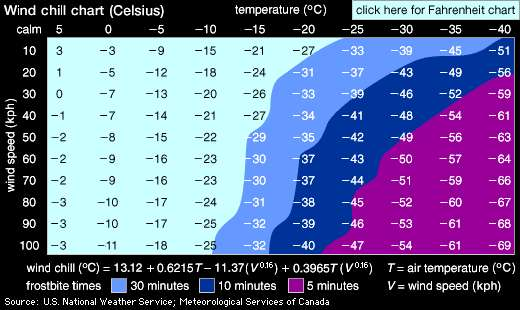
\includegraphics[width=\linewidth]{air-temperature.jpg}

\begin{enumerate}[a)]
\item Vypočtěte pomocí centrální diference parciální derivaci
$\frac {\partial W}{\partial v}$ pro teplotu $-15^\circ\mathrm C$ a rychlost větru $40\,\mathrm{km}\,\mathrm{hod}^{-1}$ a intepretujte výsledek slovně.
\item Pocitová teplota $W$ je lineární v proměnné $T$. Proto derivace $\frac{\partial W}{\partial T}$ nezávisí na $T$. Jak se tato skutečnost
  odrazí v tabulce?
  \item Odhadněte z tabulky, zda vliv větru klesá nebo roste s rychlostí větru. Potvrďte svou hypotézu analytickým výpočtem parciální derivace $\frac{\partial W}{\partial v}$ a vysvětlete fyzikálně.
\end{enumerate}

\reseni
\begin{enumerate}[a)]
\item
  $$\frac {\partial W}{\partial v}(T=-15,v=40)\approx\frac{-29-(-26)}{50-30}\frac{{}^\circ \mathrm C}{\mathrm{km}\,\mathrm{hod}^{-1}}=-0.15^\circ \mathrm C/(\mathrm{km}\,\mathrm{hod})$$
  Za podmínek, kde je $15$ stupňů pod nulou a vítr o rychlosti $40$
kilometrů za hodinu každé další zesílení větru o kilometr za hodinu
sníží pocitovou teplotu přibližně o patnáct setin stupně.
\item Neformálně: V rámci každého řádku jsou stejně velké
  skoky. Přesněji: V každém řádku je přibližně aritmetická
  posloupnost, data se mění odečtením pevné konstantny. Případné
  fluktuace od tohoto pravidla jsou způsobeny zaokrouhlením.
\item Pokud se díváme na data po sloupcích, s rostoucí silou větru
  jsou skoky menší a proto parciálni derivace podle větru s rostoucí
  rychlostí větru klesá. To potvrzuje i analytický výpočet, protože u
  rychlosti je mocnina menší než jedna a ta se po zderivání změní na
  zápornou mocninu a tím se změní charakter závislosti na rychlosti
  větru. Fyzikálně vítr odfoukává izolační mikrovrstvu vzduchu kolem
  tváře nebo těla a proto cítíme ve větším větru větší chlad. Pokud je
  vítr silný, nestačí se tato mikrovstva vytvořit ani v minimální míře
  a proto je jedno, jestli fouká hodně nebo ještě více.
\end{enumerate}
\konec

\obrazek[Wood handbook]{wood_heat_capacity.png}
\subsection{Parciální derivace, tepelná kapacita dřeva}

Vypočtěte a slovně interpretujte parciální derivaci měrné tepelné kapacity dřeva $c$ podle teploty $T$ a podle obsahu vody MC $w$ v bodě o hodnotě MC 12\% a teplotě $27^\circ\mathrm C$.

Pro obě derivace použijte dopřednou diferenci (v tabulce nejsou ekvidistatní kroky MC).

\textit{Poznámka:} Kromě dopředné diference je možné uvažovat ještě zpětou diferenci definovanou vztahem $$\frac{f(x)-f(x-h)}{h},$$ což je vlastně dopředná diference na předhozím intervalu. Ukažte, že centrální diference je průměrem dopředné a zpětné diference.

\reseni

$$\pdv{c}{T}=\frac{1.8-1.7}{47-27}=0.005 \,\mathrm{kJ}\,\mathrm{kg}^{-1}\mathrm{K}^{-2}=5 \,\mathrm{J}\,\mathrm{kg}^{-1}\mathrm{K}^{-2}$$
Tato hodnota udává, o kolik vzroste měrná tepelná kapacita dřeva dané teploty a vlhkosti při zvýšení teploty o jeden stupeň Celsia (o jeden Kelvin).

$$\pdv{c}{w}=\frac{1.9-1.7}{20-12}=0.025 \,\mathrm{kJ}\,\mathrm{kg}^{-1}\mathrm{K}^{-1}(\text{procento MC})^{-1}=25 \,\mathrm{J}\,\mathrm{kg}^{-1}\mathrm{K}^{-1}(\text{procento MC})^{-1}$$
Tato hodnota udává, o kolik vzroste měrná tepelná kapacita dřeva dané teploty a vlhkosti při zvýšení obsahu vody o jedno procento.



Průměr centrální a zpětné diference:
\begin{dmath*}
  \frac{\frac{f(x)-f(x-h)}{h} + \frac{f(x+h)-f(x)}{h}}{2}=
  \frac{\frac{f(x)-f(x-h)+f(x+h)-f(x)}{h}}{2}=
\frac{f(x+h)-f(x-h)}{2h}
\end{dmath*}

\konec

\stranka
\subsection{Veličiny z rovnice vedení tepla}

\begin{multicols}2
V případech, kdy je při tepelné výměně nutno uvažovat vedení tepla (vysoké Biotovo číslo), modelujeme změnu teploty podle rovnice vedení tepla, kterou jsme na přednášce odvodili pro jednorozměrný případ ve tvaru
$$\varrho c \frac{\partial T}{\partial t}=\frac{\partial}{\partial x}\Bigl(\lambda\frac{\partial T}{\partial x}\Bigr).$$  Typickým případem vedení tepla v jedné dimenzi je vedení tepla ve stěně. 

Uvažujme jednorozměrnou úlohu s vedením tepla. Osa $x$ směřuje doprava, teplota v~bodě $x$ a čase $t$ je $T(x,t)$ ve stupních Celsia. Tok tepla v čase $t$ a v bodě $x$ je $q(x,t)$ v~joulech za sekundu. Kladný tok je ve směru osy $x$.
Podle Fourierova zákona je $$q=-\lambda \frac{\partial T}{\partial x}.$$

Tyč má teplotu $0\,^{\circ}\mathrm{C}$, pravý konec udržujeme na této teplotě, levý konec ohříváme na $20\,^{\circ}\mathrm{C}$ a udržujeme na této teplotě. Ve zbytku tyče (stěny) se postupně nastolí rovnováha vlivem vedení tepla.

\vspace*{-5pt}
Vyjádřete následující veličiny a určete jejich znaménko.

\vspace*{-15pt}
\begin{enumerate}[a)]\itemsep -2 pt
\item Rychlost, s jakou v daném místě a čase roste teplota jako funkce času.
\item Rychlost, s jakou v daném místě a čase roste teplota jako funkce polohy, tj. jak rychle  roste teplota směrem doprava.
\item Rychlost, jak rychle se klesá teplota jako funkce polohy, tj. směrem doprava.
\item Rychlost, se kterou roste (směrem doprava) tok tepla jako funkce polohy.
\item Rychlost, se kterou klesá (směrem doprava) tok tepla jako funkce polohy.
\end{enumerate}
\end{multicols}

\reseni
\begin{enumerate}[a)]
\item Rychlost, s jakou v daném místě a čase roste teplota jako funkce času je $\frac {\partial T}{\partial t}$ a tato derivace je v každém bodě kladná, protože tyč se ohřívá. Po čase se asi ustálí rovnováha a derivace bude nulová, teplota se přestaně měnit. Měříme ve stupních celsia za sekundu.
  $\left[\frac {\partial T}{\partial t}\right]={}^\circ\mathrm{C}\,\mathrm{s}^{-1}$
\item Rychlost, s jakou v daném místě a čase roste teplota jako funkce polohy, tj. jak rychle se roste teplota směrem doprava, je $\frac {\partial T}{\partial x}$ a tato derivace je záporná, protože vlevo je horký konec a teplota směrem doprava klesá. Měříme ve stupních celsia na metr.
    $\left[\frac {\partial T}{\partial x}\right]={}^\circ\mathrm{C}\,\mathrm{m}^{-1}$
  \item Rychlost, jak rychle se klesá teplota jako funkce polohy, tj. směrem doprava, je $-\frac {\partial T}{\partial x}$ a tato veličina je kladná, protože vlevo je horký konec a teplota směrem doprava opravdu klesá. Měříme ve stupních celsia na metr.
        $\left[-\frac {\partial T}{\partial x}\right]={}^\circ\mathrm{C}\,\mathrm{m}^{-1}$

\item Rychlost, se kterou roste (směrem doprava) tok tepla jako funkce polohy je $\frac {\partial q}{\partial x}$. Teplo teče doprava a přitom se spotřebovává, protože se ohřívá tyč. Proto tok klesá a parciální derivace je záporná.
  Měříme v joulech za sekundu na metr.
          $\left[\frac {\partial q}{\partial x}\right]=\mathrm{J}\,\mathrm{s}^{-1}\,\mathrm{m}^{-1}$
\item Rychlost, se kterou klesá (směrem doprava) tok tepla jako funkce polohy je $-\frac {\partial q}{\partial x}$ a tato veličina je kladná, což plyne z předchozího bodu a z toho, že jsme změnili znaménko.
  Měříme v joulech za sekundu na metr.
            $\left[-\frac {\partial q}{\partial x}\right]=\mathrm{J}\,\mathrm{s}^{-1}\,\mathrm{m}^{-1}$ Tato veličina udává, kolik tepla se za jednotku času ubude v toku na metrovém úseku tyče. Ze zákona zachování energie se toto teplo nemůže ``ztratit'', ale použije se na zvýšení teploty, což je vyjádřeno právě v rovnici vedení tepla.
\end{enumerate}

\konec




%\obrazek{stena_cihly}
\subsection{Okrajové podmínky pro rovnici vedení tepla}

\begin{multicols}2
  K modelu stěny pomocí rovnice vedení tepla je ještě nutné přidat podmínky související s počátečním stavem (počáteční podmínky) a s~chováním na okrajích (okrajové podmínky).

  Nechť stěna je na intervalu $x\in[0,L]$, $x=0$ je vnitřní okraj a $x=L$ je vnější okraj. Výraz $-k\frac{\partial T}{\partial x}$ udává tok tepla ve směru osy $x$. Tok ve směru osy $x$ má kladné znaménko. Naformulujte okrajové podmínky v následujících scénářích.
\begin{enumerate}[a)]\itemsep 0 pt
\item Z venku dokonale izolovaná stěna. Na hranici $x=L$ nedochází k toku tepla.
\item Vnitřní část stěny je udržovaná na konstantní teplotě $T=23^\circ \mathrm C$.
\item Stěna je zvenku osvětlená a zahřívaná Sluncem. Na vnější hranici je konstantní tok tepla směrem do stěny.
\item Stěna je zvenku ochlazována prouděním vzduchu. Tok tepla mezi stěnou a okolím je úměrný rozdílu teplot stěny a okolí.
% \item Stěna je zevnitř zahřívaná infrazářičem. Na vnitřní straně stěny je konstantní tok tepla směrem do stěny.
\item Stěna je zevnitř ohřívána prouděním vzduchu od radiátorů. Tok tepla mezi stěnou a okolím je úměrný rozdílu teplot stěny a okolí.
\end{enumerate}
\textit{Zpracováno podle Cengel: Mass and heat transfer.} 
\end{multicols}

\reseni

\begin{enumerate}[a)]
\item $\frac{\partial T}{\partial x}(L)=0$
\item $T(0)=23$
\item $-k\frac{\partial T}{\partial x}(L)=-Q$, kde $Q$ je teplo za jednotku času dodané ze Slunce. Jedná se výkon Slunce dopadající na stěnu vynásobený koeficientem absorbce, protože část tepelného výkonu se odráží. Záporné znaménko je proto, že teplo teče do stěny, tj. proti směru osy $x$.
\item $-k\frac{\partial T}{\partial x}(L)=h(T-T_{\text{okolí}})$, kde $h$ je koeficient přestupu tepla.
% \item $-k\frac{\partial T}{\partial x}(L)=Q$, kde $Q$ je teplo za jednotku času dodané z infrazářiče. Jedná se výkon dopadající na stěnu vynásobený koeficientem absorbce. Teplo teče do stěny, tj. ve směru osy $x$.
\item $-k\frac{\partial T}{\partial x}(0)=h(T_{\text{místnost}}-T)$, kde $h$ je koeficient přestupu tepla.
  Všimněte si, že poslední dvě podmínky se liší znaménkem u veličiny $T$. To proto, že v jednom případě je kladný směr toku tepla do materiálu a jednou z materiálu. Pokud chceme mít popis jednotný, nebo nezávislý na zvolené souřadné soustavě, formulujeme podmínky pro tok tepla ven z materiálu. Tento tok získáme tak, že tok tepla vynásobíme skalárně s jednotkovým vektorem směřujícím ven z materiálu kolmo na jeho povrch. V tomto případě by pro tok ze stěny do místnosti bylo $k\frac{\partial T}{\partial x}(0)=h(T-T_{\text{místnost}})$. Tento tok by byl záporný, protože ve skutečnosti teplo uniká z místnosti stěnou ven.
\end{enumerate}
\konec


\section{Gradient}

\subsection{Parciální derivace, gradient}

Určete gradient funkcí $z=ax^2y-2xy^2$ a $h=\frac {ax}{y^2}+5x^3y^2$, kde $a\in\mathbb R$ je reálný parametr.

\reseni
\begin{align*}
  \pdv{z}{x} &= 2axy-2y^2\\
  \pdv{z}{y} &= ax^2-4xy\\
  \nabla z &= (2axy-2y^2, ax^2-4xy) = (2axy-2y^2)\vec \imath + (ax^2-4xy)\vec \jmath\\
  \pdv{h}{x} &= \frac a{y^2}+15x^2y^2\\
  \pdv{h}{y} &= ax(-2)y^{-3}+10x^3y=-\frac{2ax}{y^3}+10x^3y\\
  \nabla h &= \left(\frac a{y^2}+15x^2y^2, -\frac{2ax}{y^3}+10x^3y\right) = \left(\frac a{y^2}+15x^2y^2\right)\vec \imath + \left(-\frac{2ax}{y^3}+10x^3y\right)\vec \jmath
\end{align*}
\konec

\subsection{Gradient funkce s vrstevnicemi ve tvaru kružnic}

Určete gradient funkce $z=x^2+y^2$ a zkontrolujte, že je v každém bodě kolmý ke kružnici se středem v počátku. Využijte toho, že spojnice bodu na kružnici se středem kružnice je kolmá k této kružnici. 

\reseni
\begin{align*}
  \pdv{z}{x} &= 2x\\
  \pdv{z}{y} &= 2y\\
  \nabla z &= (2x, 2y) = 2x\vec \imath + 2y\vec \jmath
\end{align*}
Vektor $(2x,2y)$ v bodě $(x,y)$ míří směrem od počátku, tj ve směru spojnice se středem a tedy je kolmý k vrstevnici.
\konec



\subsection{Gradient funkce s paprskovitými vrstevnicemi}

Určete gradient funkce $z=\mathop{\mathrm{arctg}} \frac yx$ a zkontrolujte, že je v každém bodě tečný ke kružnici se středem v počátku. Využijte toho, že tečna je kolmá na poloměr.


\reseni
\begin{align*}
  \pdv{z}{x} &= \frac1{1+\frac {y^2}{x^2}}y\frac {(-1)}{x^2}=-\frac{y}{x^2+y^2}\\
  \pdv{z}{y} &= \frac1{1+\frac {y^2}{x^2}}\frac 1x=\frac{x}{x^2+y^2}\\
  \nabla z &=  \left(-\frac{y}{x^2+y^2},\frac{x}{x^2+y^2}\right)= \frac{1}{x^2+y^2} (-y,x)
\end{align*}
Vektor $(-y,x)$ v bodě $(x,y)$ je kolmý k vektoru $(x,y)$ a míří směrem od počátku, tj. k~poloměru. Proto je tečný ke kružnici.
\konec



\obrazek{blizzard.jpg}

\subsection{Linearizace pocitové teploty}

Pocitová teplota $W$ z minulého cvičení má v bodě odpovídajícím teplotě $T=-11{}^\circ\mathrm C$ a rcyhlosti větru $v=26\,\mathrm {km}\,\mathrm{hod}^{-1}$ má hodnotu $$W=-20.2 ^\circ\mathrm C$$ a parciální derivace $$\pdv{W}{v}=-0.163 ^\circ\mathrm C\, \mathrm {hod}\,\mathrm{km}^{-1}$$ a
$$\pdv{W}{T}=1.289.$$ Najděte pomocí lineární aproximace vzorec pro pocitovou teplotu v okolí tohoto bodu.

\reseni

Přímým použitím vzorce pro lineární aproximaci dostáváme
\begin{dmath*}
W=-20.2+1.289(T-(-11))-0.163(v-26)=-20.2+1.289(T+11)-0.163(v-26),
\end{dmath*}
přičemž všechny veličiny dostazujeme v jednotkách SI (stupně Celsia a kilometry za hodinu).

\konec


\obrazek[Wood handbook]{anatomicke_smery_dreva.png}

\subsection{Parciální derivace, gradient a násobení matic}

Vypočtěte gradient funkce $$T=10-\sqrt{x^2+y^2}.$$ Ukažte, že vrstevnice
této funkce jsou kružnice se středem v počátku, nakreslete obrázek s
těmito vrstevnicemi a vyznačte do tohoto obrázku gradienty v bodech
$A=(0,1)$, $B=(1,0)$ a $C=(1,1)$

Uvažujte součinitel tepelné vodivosti $$\lambda =
\begin{pmatrix}
  2&0\\0&3
\end{pmatrix}$$
a vypočtěte tok tepla v bodech $A$, $B$, $C$. Porovnejte směr tohoto toku se směrem gradientu a vysvětlete svá pozorování. Snaží se matice usměrnit teplo do  směru osy $x$ nebo do  směru osy $y$? Odpovídá situace spíše dřevu s podélným směrem v ose $x$ nebo v ose $y$?


\reseni

Platí $$\pdv{T}{x}=-\frac 12 (x^2+y^2)^{-\frac 12}(2x)=-\frac{x}{\sqrt{x^2+y^2}}$$
a ze symetrie 
$$\pdv{T}{y}=-\frac{y}{\sqrt{x^2+y^2}}.$$
Odsud $$\nabla T=\qty(-\frac{x}{\sqrt{x^2+y^2}},-\frac{y}{\sqrt{x^2+y^2}})^T
=
-\frac 1{\sqrt{x^2+y^2}}(x,y)^T.$$
Tok tepla je
$$\vec q=-\lambda \nabla T=\frac 1{\sqrt{x^2+y^2}}\begin{pmatrix}
  2&0\\0&3
\end{pmatrix}
\begin{pmatrix}
  x\\y
\end{pmatrix}
=\frac 1{\sqrt{x^2+y^2}} \begin{pmatrix}
  2x\\3y
\end{pmatrix}
$$
Dosazením dostáváme $\vec q(A)=(0,3)^T$, $\vec q(B)=(2,0)^T$, $\vec q(C)=\frac 1{\sqrt{2}}(2,3)^T$. Porovnáním s gradientem $\nabla T(A)=-(0,1)^T$, $\nabla T(B)=-(1,0)^T$ a $\nabla T(C)=-\frac 1{\sqrt 2}(1,1)^T$ vidíme, že v bodech $A$  a $B$ je tok proti směru gradientu, v bodě $C$ se tok stáčí do směru osy $y$. Protože ve ose $y$ má dřevo větší vodivost, jedná se o podélný směr. To je ale vlastně vidět už ze zadané matice.

\konec


\subsection{Tečná rovina atd.}

Pro funkci $f(x,y)=x^2+\frac x{y^2}-6$ najděte
\begin{enumerate}[a)]
\item gradient, 
\item gradient v bodě $(2,1)$,
\item lineární aproximaci v bodě $(2,1)$,
\item tečnou rovinu v bodě $(2,1)$,
\item rovnici vrstevnice bodem $(2,1)$ a rovnici tečny k vrstevnici tímto bodem,
\item explicitní vyjádření funkce dané v okolí bodu $(2,1)$ implicitně rovnicí $f(x,y)=0$,
\item lineární aproximace v okolí bodu $x=2$ pro funkci získanou v předchozím bodu.
\end{enumerate}

\reseni
\begin{enumerate}[a)]
\item $\nabla f=\left(2x+\frac 1{y^2},-2\frac x{y^3}\right)$
\item $\nabla f(2,1)=(5,-4)$
\item $f(x,y)\approx 5(x-2)-4(y-1)$
\item $z= 5(x-2)-4(y-1)$
\item Rovnice vrstevnice je $$x^2+\frac x{y^2}-6=0$$
  a tečna $$5(x-2)-4(y-1)=0,$$ tj. $$5x-4y-6=0.$$
\item Postupnými úpravami a výběrem správného znaménka po vyřešení kvadratické rovnice vzhledem k $y$ dostáváme
  $$
  \begin{aligned}
    x^2+\frac x{y^2}-6&=0\\
        \frac x{y^2}&=6-x^2\\
        y^2&=\frac{x}{6-x^2}\\
        y&=\sqrt{\frac{x}{6-x^2}}\\
  \end{aligned}
$$
\item Z rovnice tečny k vrstevnici $$5(x-2)-4(y-1)=0$$
  dostáváme $$y=1+\frac 54 (x-2)$$
  a proto
  $$\sqrt{\frac{x}{6-x^2}}\approx 1+\frac 54 (x-2)$$ v okolí $x=2$.
\end{enumerate}

\konec


\stranka
\section{Divergence, rovnice vedení tepla}


\subsection{Divegrence vektorového pole}

\begin{enumerate}[a)]
\item Vypočtěte divergenci vektorového pole
  $$\vec F=x^2y\vec \imath + (x+y^2)\vec \jmath.$$
\item Zakreslete do obrázku směr toku vektorového pole v bodě $(2,1)$. 
\item Vypočtěte divergenci vektorového pole v bodě $(2,1)$ a podle toho, zda je kladná nebo záporná rozhodněte, zda se tok v daném bodě zhušťuje nebo řídne.
\item Předpokládejme, že dané vektorové pole reprezentuje stacionární tok. Je v bodě $(2,1)$ zdroj nebo spotřebič?
\end{enumerate}
\reseni

\begin{enumerate}[a)]
\item $\nabla \cdot \vec F=\pdv{x}(x^2y)+\pdv{y}(x+y^2)
=2xy+(0+2y)=2y(x+1)$
\item $\vec F(2,1)=2^2\cdot 1\vec \cdot \imath + (2+1^2)\vec \jmath=4\vec\imath+3\vec\jmath=(4,3)$, tj. vektorové pole teče směrem doprava nahoru směrem daným směrnicí $0.75$, tj. pod úhlem menším než $45^\circ$.
\item $\nabla\cdot\vec F(2,1)=2\cdot 1 \cdot(2+1)=6>0$. Divergence je kladná a proto se tok zahušťuje.
\item Zdroj (kladná divergence).
\end{enumerate}
\konec

\subsection{Divegrence vektorového pole s parametrem}

\begin{enumerate}[a)]
\item Vypočtěte divergenci vektorového pole
  $$\vec F=ax^3y^2\vec \imath + 3x^2y\vec \jmath,$$ kde
  $a\in\mathbb R$ je reálný parametr.
\item Určete hodnotu parametru $a$ tak, aby pole bylo v bodě $(-1,2)$ nezřídlové, tj. aby mělo nulovou divergenci v bodě $(-1,2)$.
\end{enumerate}
\reseni

\begin{enumerate}[a)]
\item $\nabla \cdot \vec F=\pdv{x}(ax^3y^2)+\pdv{y}(3x^2y)
=3ax^2y^2+3x^2=3x^2(ay^2+1)$
\item $\nabla \cdot \vec F (-1,2)=3(-1)^2(a\cdot 2^2+1)=3(4a+1) $ a $\nabla \cdot \vec F (-1,2)=0$ pokud $3(4a+1)=0$, tj. $a=-\frac 14$.
\end{enumerate}
\konec

\obrazek{drevo_textura.jpg}

\subsection{Rovnice vedení tepla v dvourozměrném materiálu}

Teplota ve dvourozměrné desce pro $0\leq x\leq 10$ a $0\leq y\leq 10$ zachycené v určitém okamžiku termokamerou je popsána rovnicí
  $$T(x,y)=(x+2y)^2+x^3.$$
  Rozměry jsou v centimetrech, teplota ve stupních Celsia. (Formálně to nevychází, ale ke každému členu můžeme dodat konstantu, která jeho rozměr opraví. Pro jednoduchost tuto komplikaci vynecháme.)

\begin{enumerate}[a)]
\item Vypočtěte gradient $\nabla T$  a tok tepla $-k \cdot \nabla T.$
Součinitel tepelné vodivosti (v jednotkách kompatibilních se zadáním) je $k=
  \begin{pmatrix}
    5 & 1\\1&4
  \end{pmatrix}.
$ 
\item Určete, zda na levém okraji desky teče teplo dovnitř desky nebo z desky ven.
\item Vypočtěte divergenci toku tepla, tj. $\nabla\cdot(-k \cdot \nabla T).$
\item V desce nejsou zdroje tepla. Ochlazuje se deska uprostřed, nebo otepluje?
\end{enumerate}

\reseni
\begin{enumerate}[a)]
\item $\nabla T=\qty(2(x+2y)+3x^2,4(x+2y))^T$,\\
  $-k\cdot \nabla T=-
  \begin{pmatrix}
    5&1\\1&4
  \end{pmatrix}
  \begin{pmatrix}
    2(x+2y)+3x^2\\4(x+2y)
  \end{pmatrix}
  =-
  \begin{pmatrix}
    14(x+2y)+15x^2\\18(x+2y)+3x^2
  \end{pmatrix}
$
\item
  $-k\cdot \nabla T (x=0)=
  \begin{pmatrix}
    -28y\\-36y
  \end{pmatrix}
  $
  
  Na levém okraji desky je $y>0$ a proto $(-28y)<0$. Tok míří doleva a teplo teče na tomto okraji ven z desky.
\item $\nabla \cdot (-k\cdot \nabla T )=\pdv{x}(-14(x+2y)-15x^2)+\pdv{y}(-18(x+2y)-3x^2)=-30x-50$
  \item $\nabla \cdot (-k\cdot \nabla T )(x=5,y=5)=-200$, tok tepla se zmenšuje a protože jde o stav bez zdrojů, teplo se v daném místě akumuluje a deska se proto otepluje.
\end{enumerate}
\konec

% var('x,y')
% k=matrix([[5,1],[1,4]])
% T(x,y)=(x+2*y)^2+x^3
% show(T.gradient())
% show(-k*T.gradient())
% show(-k*T.gradient()(x=0))
% show((-k*T.gradient())[0].diff(x)+(-k*T.gradient())[1].diff(y))

\subsection{Vedení tepla v různých materiálech}

\begin{enumerate}[a)]
\item Zapište rovnici vedení tepla v trojrozměrném izotropním a v
  trojrozměrném ortotropním materiálu. Ve druhém případě volte osy ve
  směru vlastních vektorů.
\item Napište, jak je možné zjednodušit rovnice z předchozího bodu,
  pokud jsou materiálové konstanty nezávislé na poloze (homogenní
  materiál) a na teplotě (lineární materiál).
\end{enumerate}

\reseni
\begin{enumerate}[a)]
\item Izotropní: $\varrho c \pdv{T}{t} = 
\pdv{x}(k\pdv{T}{x})
+\pdv{y}(k\pdv{T}{y})
+\pdv{z}(k\pdv{T}{z})$

  Ortotropní:
 $\varrho c \pdv{T}{t} = 
\pdv{x}(k_x\pdv{T}{x})
+\pdv{y}(k_y\pdv{T}{y})
+\pdv{z}(k_z\pdv{T}{z})
$
\item Izotropní: $\varrho c \pdv{T}{t} = 
k\left(\pdv[2]{T}{x} + \pdv[2]{T}{y} + \pdv[2]{T}{z}\right)
$

  Ortotropní:
 $\varrho c \pdv{T}{t} = 
k_x\pdv[2]{T}{x}
+k_y\pdv[2]{T}{y}
+k_z\pdv[2]{T}{z}
$
\end{enumerate}
\konec

\section{Rotace, kmenová funkce gradientu}

\subsection{Divergence a rotace 2D funkce s parametrem}
Vypočtěte divergenci a rotaci funkce $\vec F=ax^2y^3\vec \imath + (x^2+y)\vec\jmath$.

\reseni

$$\nabla\cdot \vec F=\pdv{x}(ax^2y^3)+\pdv{y}(x^2+y)=2axy^3+1$$

 $$\curl \vec F=
 \begin{vmatrix}
   \vec\imath & \vec \jmath & \vec k\\
   \pdv{x} & \pdv{y} & \pdv{z} \\
   ax^2y^3 & x^2+y & 0
 \end{vmatrix}
 =\vec k(2x-3ax^2y^2)
 $$

\konec


\subsection{Nalezení kmenové funkce 1/3}

Pro vektorové pole $$\frac 45 x y^3\vec \imath + \frac 65x^2y^2\vec\jmath$$ najděte funkci $\varphi$ tak, že zadané vektorové pole je rovno gradientu $\nabla \varphi.$

\subsection{Nalezení kmenové funkce 2/3}

Pro vektorové pole $$\left(x^2+\frac 45 x y^3\right)\vec \imath + \left(\frac 65x^2y^2+y\right)\vec\jmath$$ najděte funkci $\varphi$ tak, že zadané vektorové pole je rovno gradientu $\nabla \varphi.$

\subsection{Nalezení kmenové funkce 3/3}

Pro vektorové pole $$\left(y+\frac 45 x y^3\right)\vec \imath + \left(\frac 65x^2y^2+x^2\right)\vec\jmath$$ najděte funkci $\varphi$ tak, že zadané vektorové pole je rovno gradientu $\nabla \varphi.$




\section{Křivkové integrály}




\section{Dvojné integrály}


\subsection{Jacobiho matice pro polární souřadnice}

Najděte Jacobiho matici a její determinant pro transformaci 
\begin{equation*}
  \begin{aligned}
    x&=r\cos \varphi\\
    y&=r\sin \varphi
  \end{aligned}
\end{equation*}
mezi polárními a kartézskými souřadnicemi.


\section{Greenova věta, křivkový integrál pomocí potenciálu}

\subsection{Křivkový integrál pomocí kmenové funkce}

Určete, pro jako hodnotu parametru $a\in \mathbb R$ křivkový integrál $$\int_C ax^2y\,\mathrm dx+(x^3+1)\,\mathrm dy$$ nezávisí na integrační cestě v $\mathbb R^2$. Najděte kmenovou funkci příáslušného vektorového pole a vypočtěte křivkový integrál po křivce z bodu $[0,0]$ do bodu $[1,2]$.

\reseni

Podmínka pro nezávislost na integrační cestě je $$
\begin{aligned}
  \pdv{y}(ax^2y)&=\pdv{x}(x^3+1)\\
  ax^2&=3x^2\\
  a&=3
\end{aligned}
$$
Kmenová fukce $\varphi(x,y)$ vektorového pole $\vec F=(3x^2y,x^3+1)$ splňuje
$$
\begin{aligned}
  \pdv{\varphi}{x}&=3x^2y \\  \pdv{\varphi}{y}&=x^3+1.
\end{aligned}
$$
Integrací dostáváme
$$
\begin{aligned}
  \varphi &= \int 3x^2y\,\mathrm dx=x^3y+C_1(y)\\
  \varphi &= \int x^3+1\,\mathrm dy=x^3y+y+C_2(x)
\end{aligned}
$$
Porovnáním dostáváme kenovou funkci $$\varphi (x,y)=x^3y+y+C,$$ kde $C$ je integrační konstanta. Integrál po křivce (tvar není důležitý, vzhledem k nezávislosti na integrační cestě stačí počáteční a koncový bod) je
$$\int _C \vec F\mathrm d\vec r=\varphi(1,1)-\varphi(0,0)=1+1-0=2.$$

\konec


\section{Diferenciální rovnice I}

\section{Diferenciální rovnice II}

\section{Autonomní systémy}

\section{Diferenciální rovnice druhého řádu}

\section{Více integrálů}

\section{Více diferenciálních rovnic}

\section{Shrnutí}






